\chapter{Unit Tests}

\section{10 Unit Tests}

\hyphenation{DirectionTest}
\begin{table}[H]
    \centering
    \begin{tabular}{|p{7cm}|p{7cm}|}
      \hline
      \textbf{Unit Test} & \textbf{Beschreibung} \\
      \hline
      1. VectorTest\#dotTest & Testet \textit{dotTest}-Funktion der Klasse \textit{Vector} darauf, ob sie korrekt Skalarprodukte berechnet \\
      \hline
      2. VectorTest\#lengthTest & Testet \textit{length}-Funktion der Klasse \textit{Vector} darauf, ob sie korrekt Vektorlängen berechnet \\
      \hline
      3. VectorTest\#getClockwiseAngleFromTest & Testet \textit{getClockwiseAngleFrom}-Funktion der Klasse \textit{Vector} darauf, ob sie korrekt Winkel zwischen zwei Vektoren berechnet \\
      \hline
      4. NumericTest\#clampTest & Testet \textit{clamp}-Funktion der Klasse \textit{Numeric} darauf, ob sie korrekt Werte in einem gegebenen Intervall einschließt \\
      \hline
      5. EntityTest\#getPreferredMovement DirectionTest & Testet \textit{getPreferredMovementDirection}-Funktion der Klasse \textit{Enemy} darauf, ob sie korrekt eine Bewegung aufgrund der Position des Spielers wählt \\
      \hline
      6. RoomGridTest\#fitsTest & Testet \textit{fits}-Funktion der Klasse \textit{RoomGrid} darauf, ob sie korrekt feststellen kann, ob ein Raum noch auf die Spielkarte passt \\
      \hline
      7. RoomPositionTest\#getMaxDistanceAlongAnyAxisTest & Testet \textit{getMaxDistanceAlongAnyAxis}-Funktion der Klasse \textit{RoomPosition} darauf, ob sie korrekt die maximale Entfernung entlang einer von beiden Axen von einem Punkt zum anderen berechnen kann \\
      \hline
      8. CollectionSelectorTest\#randomSubset Test & Testet \textit{random}-Funktion der Klasse \textit{CollectionSelector} darauf, ob sie korrekt Teilmengen der Auswahl selektiert \\
      \hline
    \end{tabular}
    \caption{Unit Tests mit Beschreibung I}
\end{table}

\begin{table}[H]
    \centering
    \begin{tabular}{|p{7cm}|p{7cm}|}
      \hline
      \textbf{Unit Test} & \textbf{Beschreibung} \\
      \hline
      9. GameStateTest\#movementTest & Testet die Klasse \textit{Game} mithilfe des \textit{KeyInputHandlerFake}, ob der Spielzustand nach beliebigen Eingabesequenzen korrekt ist \\
      \hline
      10. RepositoryTest\#loadAndSaveRobustnessTest & Testet die Robustheit, insbesondere das \textit{Exception}-Verhalten der \textit{load()}- und \textit{save()}-Funktionen der Klasse \textit{Game} mithilfe des \textit{GameRepositoryFake} \\
      \hline
    \end{tabular}
    \caption{Unit Tests mit Beschreibung II}
\end{table}

\section{ATRIP: Automatic}
Der Begriff \textit{Automatic} bezieht sich auf die automatische
Ausführung von Unit Tests. Dies kann mit herkömmlichen Test-Frameworks
wie etwa \textit{JUnit5} erreicht werden. 

Dabei können Methoden eigens zum Testen erstellt werden, welche mit
\textit{@Test} annotiert werden. Innerhalb der IDE (z.B. IntelliJ)
können sie dann über einen Befehl oder Knopfdruck einzeln oder im
Gesamten ausgeführt werden.

Die Tests sind so konzipiert, dass sie nicht andere Durchläufe beeinflussen.
Sie sind also unabhängig von einander (\textit{Independence}) und 
wiederholbar (\textit{Repeatability}). Das führt zu nachvollziehbaren
Ergebnissen. Zudem besitzen die Tests keine externen Abhängigkeiten.

Zum Schluss gibt JUnit eine Zusammenfassung aus. Diese beschreibt die
erfolgreichen und fehlgeschlagenen Tests.
\pagebreak

\section{ATRIP: Thorough}
\subsection*{Positiv-Beispiel}
Der nachfolgende Code-Ausschnitt zeigt das Positiv-Beispiel zum
\textit{Thorough}-Aspekt. Hierbei wird die
\textit{getClockwiseAngleFromTest()}-Funktion der Klasse
\textit{Vector} getestet, welche den Winkel im Uhrzeigersinn 
zwischen zwei Vektoren berechnet. Dabei gibt es einige verschiedene
Möglichkeiten. Diese hängen unter anderem von der Definitionsreihenfolge
der beiden involvierten Vektoren ab. Dabei beginnt die Winkelmessung
beim zweiten angegebenen Vektor und läuft bis zum ersten Vektor im
Uhrzeigersinn. Es gibt zudem auch Fälle, in denen die Berechnung
fehlschlägt, etwa dann wenn ein Vektor der Nullvektor ist.

Der Test ist \textit{Thorough}, da er als \textit{ParameterizedTest}
umgesetzt ist und die Eingabe-Quelle \textit{getClockwiseAngleFromArguments()}
eine gründliche Stichprobe möglicher Fälle bereitstellt. Dabei werden
etwa Standardfälle in einigen Ausführungen und Definitionsreihenfolgen
ausprobiert, sowie unübliche Fälle, Edge Cases und pathologische Fälle.

\lstset{ 
    language=Java,
    basicstyle=\fontfamily{pcr}\selectfont\footnotesize,
    keywordstyle=\color{purple},
    numberstyle=\tiny,    
    showspaces=false,
    showstringspaces=false,
    showtabs=false, 
    frame=single,
    tabsize=2,
    rulesepcolor=\color{gray},
    rulecolor=\color{black},
    captionpos=b,
    breaklines=true,
    breakatwhitespace=false, 
}

\vspace{0.5cm}
\begin{lstlisting}[caption={ATRIP: Thorough / Positiv}]
    @ParameterizedTest
    @MethodSource("getClockwiseAngleFromArguments")
    void getClockwiseAngleFromTest(Vector to, Vector from, double angle) {
        assertEquals(angle, to.getClockwiseAngleFrom(from));
    }
    
    private static List<Arguments> getClockwiseAngleFromArguments() {
        return List.of(
                Arguments.of(Vector.UP, Vector.UP, 0D),
                Arguments.of(Vector.RIGHT, Vector.UP, 90D),
                Arguments.of(Vector.UP, Vector.RIGHT, 270D),
                Arguments.of(Vector.LEFT, Vector.UP, 270D),
                Arguments.of(Vector.UP, Vector.LEFT, 90D),
                Arguments.of(Vector.DOWN, Vector.UP, 180D),
                Arguments.of(Vector.UP, Vector.DOWN, 180D),
                
                Arguments.of(new Vector(1, 2), new Vector(1, 2), 0D),
                Arguments.of(new Vector(1, 1), new Vector(1, -1), 90D),
                Arguments.of(new Vector(-1, 1), new Vector(1, -1), 180D),
                
                Arguments.of(new Vector(1, 1), Vector.RIGHT, 45D),
                Arguments.of(new Vector(10000, 0), Vector.UP, 90D),
                
                Arguments.of(new Vector(0, 0), Vector.UP, Double.NEGATIVE_INFINITY),
                Arguments.of(new Vector(0, 0), Vector.RIGHT, Double.NEGATIVE_INFINITY)
        );
    }
\end{lstlisting}

\subsection*{Negativ-Beispiel}
Der nachfolgende Code-Ausschnitt zeigt das Negativ-Beispiel zum
\textit{Thorough}-Aspekt. Hierbei wird die
\textit{clamp()}-Funktion der Klasse
\textit{Numeric} getestet, welche einen Wert in einem gegebenen
Intervall einschließt. Der Wert liegt entweder im Intervall oder
nimmt den Wert der jeweilig überschrittenen Intervallgrenze an.

Der Test ist nicht \textit{Thorough}, da er nur einen einzigen Fall
prüft. Dieser ist zudem trivial. Der Test hat keine Aussagekraft über
die Robustheit der \textit{clamp()}-Funktion.

\vspace{0.5cm}
\begin{lstlisting}[caption={ATRIP: Thorough / Negativ}]
    @Test
    void clampTest() {
        assertEquals(5, Numeric.clamp(0, 10, 5));
    }
\end{lstlisting}

\section{ATRIP: Professional}
\subsection*{Positiv-Beispiel}
Der nachfolgende Code-Ausschnitt zeigt das Positiv-Beispiel zum
\textit{Professional}-Aspekt. Hierbei wird die
\textit{random()}-Funktion der Klasse
\textit{CollectionSelector} getestet, welche aus einer vorgegebenen
Collection versucht \textit{amount} Elemente zufällig zu wählen.
Dabei sind die gewählten Elemente unterschiedlich. Hat die Collection
zu wenige Elemente, so wird die komplette Collection zurückgegeben. 

\vspace{0.5cm}
\begin{lstlisting}[caption={ATRIP: Professional / Positiv}]
    private static final Random CONTROLLED_RANDOMNESS = new Random(69420);
    private static final List<Integer> COLLECTION = Arrays.asList(1, 2, 3, 4, 5);
    
    @ParameterizedTest
    @MethodSource("randomSubsetArguments")
    void randomSubsetTest(CollectionSelector<Integer> selector, int amount, int expectedSubsetSize) {
        Set<Integer> selection = new HashSet<>(selector.random(amount).get());
        assertEquals(expectedSubsetSize, selection.size());
        assertTrue(selector.get().containsAll(selection));
    }
    
    private static List<Arguments> randomSubsetArguments() {
        return List.of(
                Arguments.of(new CollectionSelector<>(COLLECTION, CONTROLLED_RANDOMNESS), -1, 0),
                Arguments.of(new CollectionSelector<>(COLLECTION, CONTROLLED_RANDOMNESS), 0, 0),
                Arguments.of(new CollectionSelector<>(COLLECTION, CONTROLLED_RANDOMNESS), 1, 1),
                Arguments.of(new CollectionSelector<>(COLLECTION, CONTROLLED_RANDOMNESS), 2, 2),
                Arguments.of(new CollectionSelector<>(COLLECTION, CONTROLLED_RANDOMNESS), 3, 3),
                Arguments.of(new CollectionSelector<>(COLLECTION, CONTROLLED_RANDOMNESS), 4, 4),
                Arguments.of(new CollectionSelector<>(COLLECTION, CONTROLLED_RANDOMNESS), 5, 5),
                Arguments.of(new CollectionSelector<>(COLLECTION, CONTROLLED_RANDOMNESS), 6, 5),
                Arguments.of(new CollectionSelector<>(COLLECTION, CONTROLLED_RANDOMNESS), 10000, 5)
        );
    }
\end{lstlisting}

Sie ist aus folgenden Gründen professionell:
\begin{enumerate}
    \item Es existieren keine Code-Duplikationen im Test selbst.
    Alle Fälle sind in einer Eingabe-Quelle namens
    \textit{randomSubsetArguments} zusammengefasst. Dadurch kann
    nachvollzogen werden, an welchen Stellen der Test fehlschlägt.
    Zudem ist die Logik sehr viel einfacher zu erkennen und
    nachzuvollziehen.
    \item Durch den \textit{ParameterizedTest} ist zudem einfacher zu
    erkennen, ob alle wichtigen Fälle abgedeckt sind und die Funktion
    gründlich untersucht wurde.
    \item Durch fehlende Duplikation kann die Test-Funktion sich auf
    die grundlegende Mechanik beschränken. Variablennamen bleiben
    dadurch verständlich, weil keine Alternativnamen für Objekte
    gleicher Art gefunden werden müssen.
    \item Kurze aber effektive Tests vermindern das Risiko für
    \textit{Code Smells} oder Fehler im Code, wodurch die Robustheit
    und Wartbarkeit des Tests steigt.
    \item Es wird eine nicht-triviale Kernfunktion der Domäne getestet.
    Der Test sorgt damit für eine sinnvolle Erhöhung der Coverage und
    stellt sicher, dass wichtige Bestandteile für das Funktionieren
    der Gesamtanwendung selbst funktional sind.
    \item Der \textit{ParameterizedTest} erfüllt die Eigenschaft
    \textit{Thorough}.
    \item Die zu prüfende Funktion benötigt \textit{Randomness}. Für
    nachvollziehbare Ergebnisse wird der entsprechende Generator mit
    einem Seed festgesetzt.
\end{enumerate}

\subsection*{Negativ-Beispiel}
Der nachfolgende Code-Ausschnitt zeigt das Negativ-Beispiel zum
\textit{Professional}-Aspekt. Hierbei wird die
\textit{dot()}-Funktion der Klasse
\textit{Vector} getestet, welche das Skalarprodukt zwischen zwei
Vektoren berechnet.

\vspace{0.5cm}
\begin{lstlisting}[caption={ATRIP: Professional / Negativ}]
    @Test
    void dotTest() {
        Vector posA = new Vector(1, 2);
        Vector posB = new Vector(3, 4);
        Vector negC = new Vector(-1, -2);
        Vector negD = new Vector(-3, -4);
        double dot = posA.dot(posB);
        
        assertEquals(5D, posA.dot(new Vector(1, 2)));
        assertEquals(dot, posA.dot(posB));
        
        Vector e = new Vector(-1, -2);
        assertEquals(11, e.dot(negD));
        
        // [Edge Cases]
        Vector zero = new Vector(0, 0);
        assertEquals(0, posA.dot(zero));
        assertEquals(0, posB.dot(zero));
        assertEquals(0, negD.dot(zero));
    }
\end{lstlisting}

Sie ist aus folgenden Gründen nicht professionell:
\begin{enumerate}
    \item Alle Test-Fälle sind in der \textit{dotTest()}-Methode
    beschrieben. Das erschwert zum einen die Wartung, zum anderen ist
    dadurch schlecht zu erkennen, an welcher Stelle genau ein Test
    fehlgeschlagen ist. Die Beispiele sollten daher stattdessen über
    einen \textit{ParameterizedTest} umgesetzt werden.
    \item Die Instruktionsblöcke greifen teilweise ineinander. 
    Beispielsweise wird im ersten Block eine Variable benutzt, welche
    in den folgenden Blöcken genutzt wird, obwohl die Aufteilung eine
    logische Trennung suggeriert. Dadurch wird der Code
    unübersichtlicher.
    \item Die Variablenbenennung ist nicht konsequent. Anfangs werden
    Vektoren bezüglich ihrer Ausrichtung benannt, letztlich nicht mehr.
    \item Es existiert Code-Duplikation. Einmal wird
    \textit{posA.dot(posB)} in die Variable \textit{dot} geschrieben,
    danach in einem Test aber nochmals komplett ausgeschrieben. Das 
    führt zu Unübersichtlichkeit. Vermutlich hat das auch zur Prüfung,
    ob \textit{dot} sich selbst entspricht, geführt - ein trivialer
    Fall, welcher dem Test keine Aussagekraft liefert.
    \item Zudem sind Randfälle (siehe unten) mehrfach behandelt,
    obwohl die entsprechenden Stichproben logisch keinen Unterschied
    aufweisen sollten. Das spricht entweder für fehlendes Wissen oder
    Nachlässigkeit. Letztlich bringen die überflüssigen Assertions
    dem Test keine zusätzliche Aussagekraft. 
\end{enumerate}

\section{Code Coverage}

\begin{table}[H]
    \centering
    \begin{tabular}{|p{3.5cm}|p{3.5cm}|p{3.5cm}|}
        \hline
        \textbf{Class} & \textbf{Method} & \textbf{Line} \\
        \hline
        41.8\% (28/67) & 29.1\% (118/405) & 29.2\% (317/1084) \\
        \hline
    \end{tabular}
    \caption{Overall Coverage Summary}
\end{table}

Die Tabelle zeigt die Code-Coverage aller Tests über das gesamte
Projekt, aufgeschlüsselt nach Klassen, Methoden und Zeilen. Die
dargestellten Werte zeichnen eine schlechte Coverage ab. Um diese zu
erhöhen, muss noch viel Arbeit investiert werden. Bisher hat sich
die Arbeit aber hauptsächlich auf die Logik und die Design-Prinzipien
beschränkt. Über die geforderten Unit Tests ist bis dato nicht viel
passiert. Dabei ist eine hohe Coverage (häufig > 90\%) das Ziel. Sie
verspricht, dass durch entsprechende Tests schnell Bugs und neue
Fehler identifiziert werden. Zudem untermauert eine sehr gute Coverage
bei gleichzeitig sehr guter Test-Qualität entsprechend auch die hohe
Qualität des Produktes.

In diesem Fall gibt es einzelne Bereiche, die recht gute Coverage
erhalten haben. Dazu zählen die \textit{abstraction} Schicht, sowie
einige Teile in der \textit{domain} und der \textit{application}
Schicht. Aber auch hier gibt es merklich Lücken. Die \textit{plugin}
Schicht fällt der Gesamt-Coverage jedoch besonders schwer in's
Gewicht. Hier sind lediglich die Controls und die Persistenz mäßig
abgedeckt. Dabei existieren in dieser Schicht allerdings noch viele
Klassen und Funktionen, welche sich mit der Anzeige des Spiels in
der Konsole beschäftigen. Diese haben gar keine Coverage abbekommen.

\section{Fakes und Mocks}
\subsection{GameRepositoryFake}
Die nachfolgende Abbildung zeigt das UML-Diagramm des Fakes
\textit{GameRepositoryFake}. Er ist realisiert als eine weitere
Implementation des \textit{IGameRepository}-Interfaces. Dieses wird
von der Klasse \textit{Game} genutzt, um über eine Schnittstelle mit
einer Persistenz zu interagieren. Dabei können prinzipiell unerwünschte
Fehler auftreten, vor allem bei der Interaktion mit einem Dateisystem.
Diese müssen zwangsläufig behandelt werden, um ein sicheres Programm
zu gewährleisten. 

Es ist allerdings nicht zwangsläufig einfach gezielt Fehlermeldungen
zu erzeugen, um die Abdeckung der Fehlerbehandlung festzustellen. 
Daher wird auch einen Fake zurückgegriffen, welcher entsprechend
seiner Konfiguration Fehlermeldungen erzeugt und so eine fehlerhafte
Interaktion, z.B. mit einem Dateisystem simuliert.

So wurden beispielsweise die \textit{load()}- und \textit{save()}-
Funktion ausgewählt, um gefaked zu werden. Dafür gibt man entsprechend
im Test an, ob jeweilig \textit{load()} und \textit{save()} 
fehlschlagen sollen, um die Robustheit der Benutzung sicherzustellen.

\vspace{0.5cm}
\begin{figure}[H]
    \centering
    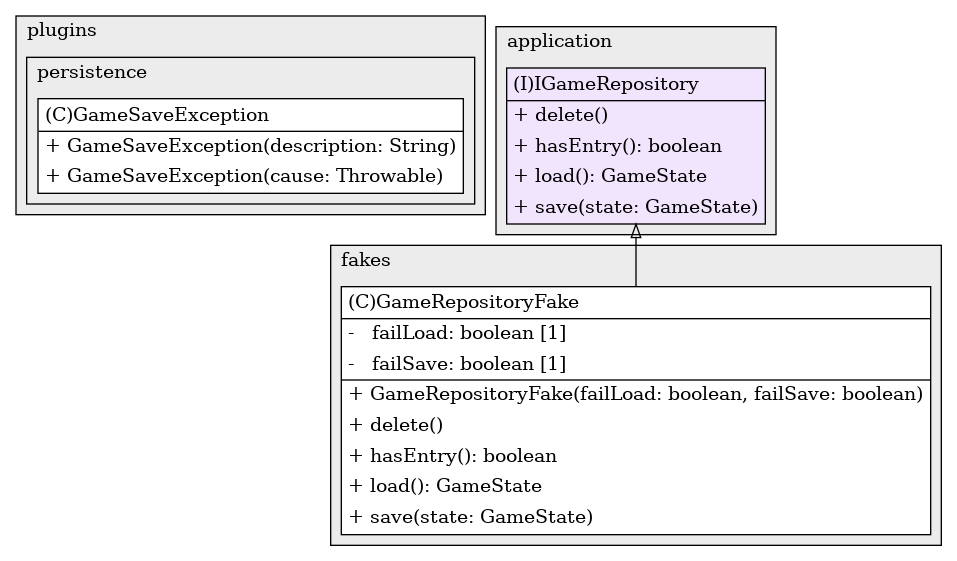
\includegraphics[width=1\linewidth]{Bilder/Visualisierung/GameRepositoryFake_structure.png}
    \caption{KeyInputHandlerFake}
\end{figure}

\subsection{KeyInputHandlerFake}

Die nachfolgende Abbildung zeigt das UML-Diagramm des Fakes
\textit{KeyInputHandlerFake}. Er ist realisiert als eine weitere
Implementation des \textit{IInteractionHandler}-Interfaces. Dieses wird
von der Klasse \textit{Game} genutzt, um über eine Schnittstelle
beliebige Aktionen entgegenzunehmen und zu verarbeiten. Um die
korrekte Verarbeitung der Aktionen sicherzustellen, wird der
Spielzustand nach einer Aktionssequenz geprüft. Dies passiert
konkret im Test \textit{GameStateTest\#movementTest}, indem die
Auswirkung von verschiedenen Aktionen auf die Bewegung und Position
des Spielers geprüft werden.

Im Normalbetrieb werden die Aktionen durch den KeyInputHandler als
Reaktion auf Tasteneingaben erzeugt. Dies ist jedoch beim Testen nicht
möglich. Der \textit{KeyInputHandlerFake} wird daher benötigt, um reale
Tasteneingaben zu simulieren und Änderungen im Spielzustand
hervorzurufen. Dafür wird für jeden Testlauf eine feste
Aktionssequenz definiert.

\vspace{0.5cm}
\begin{figure}[H]
    \centering
    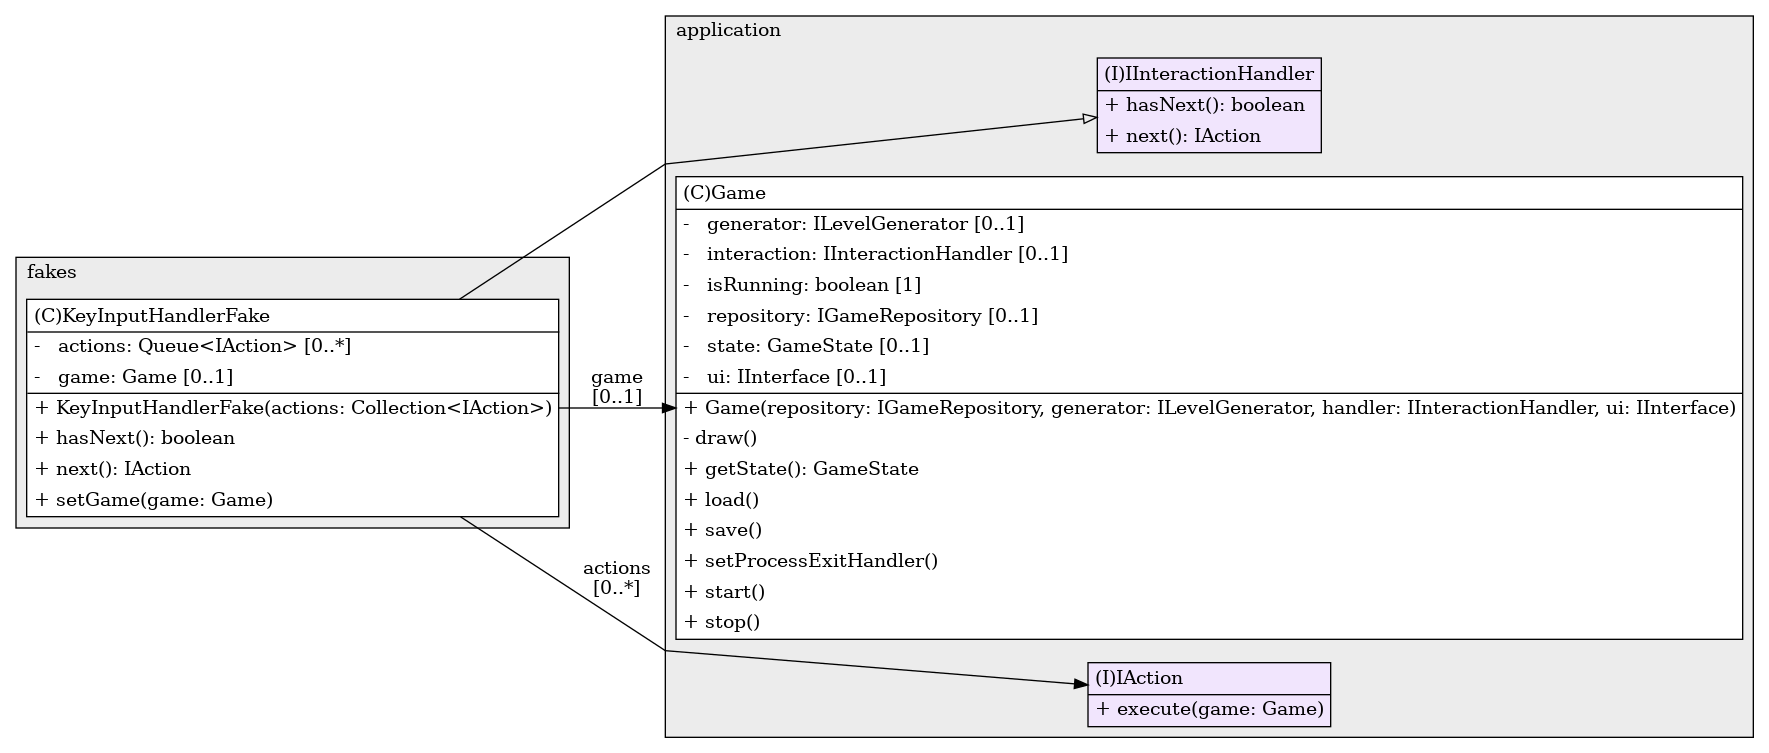
\includegraphics[width=1\linewidth]{Bilder/Visualisierung/KeyInputHandlerFake_structure.png}
    \caption{KeyInputHandlerFake}
\end{figure}
